\documentclass[preprint,12pt, a4paper]{elsarticle}

\usepackage{amsmath}
\usepackage{amssymb}
\usepackage{array}
\usepackage{booktabs}
\usepackage{color}
\usepackage{float}
\usepackage{graphicx}
\usepackage{ifpdf}
\usepackage[utf8]{inputenc}
\usepackage{keyval}
\usepackage{lineno}
\usepackage{listings}
\usepackage{longtable}
\usepackage{moresize}
\usepackage{multirow}
\usepackage{paralist}
\usepackage{rotating}
\usepackage{soul}
\usepackage{srcltx}
\usepackage{url}
\usepackage{xcolor}
\usepackage{xspace}
\usepackage{wrapfig}
\usepackage{subfig}
\usepackage{tikz}
\usepackage[export]{adjustbox} % http://ctan.org/pkg/adjustbox

\definecolor{listinggray}{gray}{0.95}
\definecolor{darkgray}{gray}{0.7}
\definecolor{commentgreen}{rgb}{0, 0.4, 0}
\definecolor{darkblue}{rgb}{0, 0, 0.6}
\definecolor{purple}{rgb}{0.6, 0, 0.6}
\definecolor{middleblue}{rgb}{0, 0, 0.75}
\definecolor{darkred}{rgb}{0.4, 0, 0}
\definecolor{brown}{rgb}{0.5, 0.5, 0}
\definecolor{dkgreen}{rgb}{0,0.5,0}
\definecolor{orange}{rgb}{1,.5,0}
\definecolor{dandelion}{cmyk}{0,0.29,0.84,0}

\usepackage[normalem]{ulem}
\makeatletter
\def\cyanuwave{\bgroup \markoverwith{\lower3.5\p@\hbox{\sixly \textcolor{cyan}{\char58}}}\ULon}
\def\reduwave{\bgroup \markoverwith{\lower3.5\p@\hbox{\sixly \textcolor{red}{\char58}}}\ULon}
\def\blueuwave{\bgroup \markoverwith{\lower3.5\p@\hbox{\sixly \textcolor{blue}{\char58}}}\ULon}
\font\sixly=lasy6 % does not re-load if already loaded, so no memory problem.
\makeatother

\def\BibTeX{{\rm B\kern-.05em{\sc i\kern-.025em b}\kern-.08em
    T\kern-.1667em\lower.7ex\hbox{E}\kern-.125emX}}

% Generate circled numbers
\newcommand*\circled[1]{\tikz[baseline=(char.base)]{
    \node[shape=circle,draw,inner sep=1pt] (char) {#1};}}
\newif\ifdraft{}
%\drafttrue{}

\ifdraft{}
  \newcommand{\amnote}[1]{ \textcolor{blue} { ***andrem: #1 }}
  \newcommand{\jhanote}[1]{ {\textcolor{red} { ***shantenu: #1 }}}
  \newcommand{\mtnote}[1]{ {\textcolor{orange} { ***matteo: #1 }}}
\else
  \newcommand{\amnote}[1]{}
  \newcommand{\jhanote}[1]{}
  \newcommand{\mtnote}[1]{}
\fi

\newcommand{\apples}{AppLeS\xspace}
\newcommand{\bj}{BigJob\xspace}
\newcommand{\computeunit}{Compute-Unit\xspace}
\newcommand{\computeunits}{Compute-Units\xspace}
\newcommand{\cloud}{cloud\xspace}
\newcommand{\clouds}{clouds\xspace}
\newcommand{\cc}{c\&c\xspace}
\newcommand{\CC}{C\&C\xspace}
\newcommand{\computedataservice}{Compute-Data Service\xspace}
\newcommand{\cu}{CU\xspace}
\newcommand{\cus}{CUs\xspace}
\newcommand{\dataunit}{Data-Unit\xspace}
\newcommand{\dataunits}{Data-Units\xspace}
\newcommand{\du}{DU\xspace}
\newcommand{\dus}{DUs\xspace}
\newcommand{\mrmg}{MR-Manager\xspace}
\newcommand{\MW}{master-worker\xspace}
\newcommand{\numrep}{8 }
\newcommand{\panda}{PanDA\xspace}
\newcommand{\pilot}{Pilot\xspace}
\newcommand{\pilots}{Pilots\xspace}
\newcommand{\pilotjob}{Pilot-Job\xspace}
\newcommand{\pilotjobs}{Pilot-Jobs\xspace}
\newcommand{\pilotcompute}{Pilot-Compute\xspace}
\newcommand{\pilotcomputes}{Pilot-Computes\xspace}
\newcommand{\pilotdata}{Pilot-Data\xspace}
\newcommand{\pilotdataservice}{Pilot-Data Service\xspace}
\newcommand{\pilotcomputeservice}{Pilot-Compute Service\xspace}
\newcommand{\prop}[1]{\textit{#1}\xspace}
\newcommand{\pilotmapreduce}{PilotMapReduce\xspace}
\newcommand{\pstar}{P*\xspace}
\newcommand{\pd}{PD\xspace}
\newcommand{\pj}{PJ\xspace}
\newcommand{\pjs}{PJs\xspace}
\newcommand{\pds}{Pilot Data Service\xspace}
\newcommand{\samplenum}{4 }
\newcommand{\su}{SU\xspace}
\newcommand{\sus}{SUs\xspace}
\newcommand{\schedulableunit}{Schedulable Unit\xspace}
\newcommand{\schedulableunits}{Schedulable Units\xspace}
\newcommand{\tmax}{\(T_{max}\)}
\newcommand{\tc}{\(T_{C}\)}
\newcommand{\tcnsp}{\(T_{C}\)}
\newcommand{\vocab}[1]{\textbf{#1}\xspace}

\newcommand{\B}[1]{\textbf{#1}\xspace}
\newcommand{\C}[1]{\textsc{#1}\xspace}
\newcommand{\F}[1]{\textbf{FIXME\@: #1}\xspace}
\newcommand{\I}[1]{\textit{#1}\xspace}
\newcommand{\T}[1]{\texttt{#1}\xspace}

\newcommand{\impterm}[1]{\texttt{#1}\xspace}

% System names
\newcommand{\bw}{\I{Blue\,Waters}}
\newcommand{\stampede}{\I{Stampede}}
\newcommand{\comet}{\I{Comet}}
\newcommand{\titan}{\I{Titan}}

% Latex Fu
\newcommand{\UPP}{\vspace*{-2.0em}}
\newcommand{\UP}{\vspace*{-1.0em}}
\newcommand{\up}{\vspace*{-0.5em}}

% Paper specific Macro's
\newcommand{\ru}{$RU$\xspace}
\newcommand{\ttc}{$ttc$}
\newcommand{\ttca}{$ttc_a$}

% Table multirows
\newcommand{\mr}[1]{\multirow{2}{*}{#1}}%
\newcommand{\mc}[2]{\multicolumn{#1}{l}{#2}}

\lstdefinestyle{myListing}{
  frame=single,   
  backgroundcolor=\color{listinggray},  
  %float=t,
  language=C,       
  basicstyle=\ttfamily \footnotesize,
  breakautoindent=true,
  breaklines=true
  tabsize=2,
  captionpos=b,  
  aboveskip=0em,
  belowskip=-2em,
}      

\lstdefinestyle{myPythonListing}{
  frame=single,   
  backgroundcolor=\color{listinggray},  
  %float=t,
  language=Python,       
  basicstyle=\ttfamily \footnotesize,
  breakautoindent=true,
  breaklines=true
  tabsize=2,
  captionpos=b,  
}

% This is now the recommended way for checking for PDFLaTeX:
\ifpdf{}
  \DeclareGraphicsExtensions{.pdf, .jpg, .tif}
\else
  \DeclareGraphicsExtensions{.eps, .jpg, .ps}
\fi

\tolerance=1000
\hyphenpenalty=10


\journal{SoftwareX}

\begin{document}
\begin{frontmatter}

% \title{Title/Name of your software}
\title{RADICAL Cybertools}

\author{A. Author}
\address{Your institute, some address}

\author{B. Author}
\address{Your institute, some address}

\author{C. Author}
\address{Your institute, some address}

\author{D. Author}
\address{Your institute, some address}

\begin{abstract}
Ca. 100 words
\end{abstract}

\begin{keyword}
%% keywords here, in the form: keyword \sep keyword
keyword 1 \sep keyword 2 \sep keyword 3

%% PACS codes here, in the form: \PACS code \sep code

%% MSC codes here, in the form: \MSC code \sep code
%% or \MSC[2008] code \sep code (2000 is the default)

\end{keyword}

\end{frontmatter}

\linenumbers{}

% The manuscript must be submitted in single column. The following
% constraints apply: 
% Word count: max. 3000.
% a.	Excluding: title, authors, affiliations, references, metadata tables.
% b.	Including: abstract, running text, captions, footnotes.
% c.	Max. 6 figures.


% ---------------------------------------------------------------------------
% Section I
% ---------------------------------------------------------------------------
\section{Motivation and significance}\label{sec:motivation}

{\em Guidelines for the authors:
\begin{enumerate}
	\item Introduce the scientific background and the motivation for
		    developing the software.
  \item Explain why the software is important, and describe the exact
        (scientific) problem(s) it solves.
	\item Indicate in what way the software has contributed (or how it will
        contribute in the future) to the process of scientific discovery;
        if available, this is to be supported by citing a research paper
        using the software.
  \item Provide a description of the experimental setting (how does the 
        user use the software?).
  \item Introduce related work in literature (cite or list algorithms 
          used, other software etc.).
\end{enumerate}}

\begin{itemize}
  \item Background:
    \begin{itemize}
      \item Growing importance of multi-task applications in multiple
      research fields.
      \item Need for scalability across several dimensions and
      infrastructures.
      \item Need for advanced capabilities like adaptivity, streaming,
      fault-tolerance, etc.
      \item The importance of supporting execution of [homo|hetero]geneous
      multi-task applications on HPC infrastructures.
      \item The rise of the pilot paradigm.
    \end{itemize}
  \item Motivations:
    \begin{itemize}
      \item Multi-task applications can be encoded into a variety of
      workflows and be executed on a variety of infrastructures.
      \item Users require flexible ways to encode workflows without having to
      buy into a specific logical representation or concrete implementation
      language.
      \item Separation between workflow description, workflow management,
      resource acquisition, workflow execution.
      \item End-to-end, monolithic and encompassing solutions do not satisfy
      these requirements.
      \item Need for an ecosystem of software modules that can be composed
      and configured depending on specific use cases.
      \item Need for rapid development of domain-specific workflow engines
      capable of supporting specific requirements without having to implement
      capabilities for resource acquisition and execution management.
      \item RCT satisfy these requirements.
    \end{itemize}
  \item Scientific relevance:
    \begin{itemize}
      \item Earth science: brief description and references
      \item Climate science: brief description and references
      \item Molecular biology: brief description and references
      \item Polar science: brief description and references
      \item \ldots
    \end{itemize}
  \item Settings:
    \begin{itemize}
      \item Python libraries supporting several deployment scenarios: local,
      local/remote, remote, multiple remote.
    \end{itemize}
  \item Related work:
    \begin{itemize}
      \item Middleware for scientific computing. Derive from: RP paper, Pilot
      paper, EnTK papers.
    \end{itemize}
\end{itemize}


% ---------------------------------------------------------------------------
% Section II
% ---------------------------------------------------------------------------
\section{Software description}\label{sec:description}

{\em Describe the software in as much as is necessary to establish a
vocabulary needed to explain its impact.}

\begin{itemize}
  % \item Currently, RTC implements four types of software system: (i)
  % workflow management system; (ii) pilot system; (iii) interoperability
  % interface; and (iv) profiler.
  % \item Building block design methodology
  \item open source development model (github, tickets, documentation,
  etc.)
\end{itemize}

The RADICAL Cyberinfrastructure tools (RCT)~\cite{web-rct} is a software
suite composed of four main components: RADICAL-SAGA
(RS)~\cite{merzky2015saga}, RADICAL-Pilot (RP)~\cite{merzky2018using} and
RADICAL-Ensemble Toolkit (EnTK)~\cite{balasubramanian2018harnessing}.

RS is a Python implementation of the OGF GFD.90 SAGA
standard~\cite{goodale2006saga}, an high-level interface to access
distributed infrastructure components like job schedulers, file transfer and
resource provisioning services. RS enables interoperability across
heterogeneous distributed infrastructures, improving on their usability and
enhancing the sustainability of services and tools.

RP is a Python implementation of the pilot paradigm and architectural
pattern~\cite{turilli2018comprehensive}. Pilot systems enables users to
submit pilot jobs to computing infrastructures and then use the resources
acquired by the pilot to execute one or more tasks. These tasks are directly
scheduled via the pilot, without having to queue in the infrastructure batch
system. RP focuses on High Performance Computing (HPC), enabling the
execution of heterogeneous workloads comprised of one or more scalar, MPI,
OpenMP, multi-process, and multi-threaded tasks. These tasks can be executed
on CPUs, GPUs and other accelerators, on the same pilot or across multiple
pilots.

EnTK is a workflow engine specialized in supporting applications composed by
an ensemble of tasks, executed both concurrently and sequentially depending
on their interdependences. EnTK promotes ensembles to a high-level
programming abstraction, providing a programming interface and execution
model specific to ensemble-based applications. EnTK is engineered for scale
and a diversity of computing platforms and runtime systems, agnostic of the
size, type and coupling of the tasks comprising the ensemble.

% RA is Python implementation of a low-level library to parse, filter and
% aggregate runtime traces of performance events. These events are timings of
% routines, message passing, and memory and CPU/GPU usage. RA supporting
% measuring duration for both single and multiple entities. For the latter,
% concurrency is taken into account so to offer precise values for global
% system behavior like total execution time and total resource utilization.
% RA implements connectors for RS, RP and EnTK\@.

RCT are designed to work both individually and as an integrated system. This
requires a ``Building Block'' approach to their design and development, based
on applying the traditional notions of modularity at component level. The
Building Block approach derives from the work on Service-oriented
Architecture and its Microservice variants, and the component-based software
development approaches where computational and compositional elements are
explicitly
separated~\cite{batory1992design,garlan1995architectural,lenz1988software,clemens1998component,schneider2000components}.
AirFlow, Oozie, Azkaban, Spark Streaming, Storm, or Kafka are examples of
tools that have a design consistent with the building blocks approach.

In our adaptation, the Building Block approach is based on four
well-understood principles: self-sufficiency, interoperability,
composability, and extensibility. A block is self-sufficient when its design
does not depend on the specificity of other building blocks; interoperable
when it can be used in diverse system architectures without semantic
modifications; composable when its interfaces enable communication and
coordination with other building blocks without syntactic modifications; and
extensible when the building's block functionalities and entities can be
extended to support new requirements or capabilities. 

The building blocks approach does not reinvent modularity, it applies it at
system level to enable composability among independent software components.
Commonly, modularity is used at function or method level, depending on the
programming paradigm. As an abstraction, modularity enables separation of
concerns by encapsulating discrete functions into semantic units (i.e.,
modules) exposed by means of a dedicated interface. Building blocks expands
upon component-based engineering to apply separation of concerns---and
therefore modularity---to each component of RCT\@.

% ---------------------------------------------------------------------------
\subsection{Software Architecture}\label{ssec:architecture}

{\em Give a short overview of the overall software architecture; provide a
pictorial component overview or similar (if possible). If necessary provide
implementation details.}

% \begin{itemize}
%   \item Create an overall architecture diagram for the whole RCT\@: RP and
%   EnTK\@. Compose this diagram from the existing diagram for each RCT
%   component, making it visually uniform.
% \end{itemize}

Ref.~\cite{merzky2015saga} details RADICAL-SAGA architecture and
capabilities. Here, we focus on RADICAL-Pilot (RP) and EnTK, first
introducing each system individually, then showing how RCT has a whole can be
composed to serve diverse use cases.

Traditionally, components of independent software systems have been difficult
to compose and reuse. While interfaces can hide implementation details
working as implementation-independent specifications of capabilities,
composability still requires semantic uniformity across interfaces. For
example, when executing multi-task applications, the notions of task or
dependency among tasks have to be uniform across components in order for them
to be composable. Obtaining this uniformity is challenging and largely
unsupported by specific formal constructs both at language and specification
level. Further, component-based engineering poses challenges in error
handling, input/output validation, effective documentation and comprehensive
testing.

Architecturally, building blocks contributes to address these challenges by
specifying state, event, error, and entities models for each block. Entities
are explicitly represented in the block's interface and used as input for
each exposed functionality. Each entity has a set of associated states,
events and errors. The order of the state is guaranteed by the implementation
(e.g., a task cannot be executed before being scheduled and scheduled before
being bound to a resource) while events are unordered but always contained
within two specific states. Errors are always associated to an entity, state
and event. Communication is decoupled from coordination, creating specific
blocks for the latter while being channel agnostic about the former.

All RCT are stand-alone, distributed systems. Architecturally, each tool
consists of one or more subsystems, each with several components. Components
are isolated into separate processes and some components are used only in
specific deployment scenarios, depending on both application requirements and
resource capabilities. Components are stateless and some of them can be
instantiated concurrently to simultaneously manage multiple entities, like
workflows, workloads, tasks or pilots. This enables scaling of throughput and
tolerance to component failure.

Concurrent components are coordinated via a dedicated communication mesh,
which introduces runtime and infrastructure-specific overheads, but improves
overall scalability of the system and lowers component complexity. Components
can have different implementations; configuration files can tailor each RCT
to specific resources types, workloads, or scaling requirements. Components
exchange data about the entities specific to each RCT and data about the
state of the components and subsystems. Each type of datum has dedicated
modules and communication channel, separating communication from coordination
while making explicit states and events of each entity.

% ------------
\subsubsection{RADICAL-Pilot}\label{sssec:arch_rp}

RP implements two main abstractions: Pilot and Compute Unit (CU). Pilots and
CUs abstract away specificities of resources and workloads, making it
possible to schedule workloads either concurrently or sequentially on
resource placeholders. Pilots are placeholders for computing resources, where
resources are represented independent from architecture and topological
details. CUs are units of work (i.e., tasks), specified as an application
executable alongside its resource and execution environment requirements.

Fig.~\ref{fig:archs}a depicts RP's architecture with two subsystems (white
boxes) and several components (purple and yellow boxes). In each subsystem,
purple components are responsible for pilots and units while yellow
components manage the communication among RP components. Subsystems can
execute locally or remotely, communicating and coordinating over TCP/IP\@,
and enabling multiple deployment scenarios. For example, users can run Client
locally, and distribute MongoDB and one or more instances of Agent on remote
computing infrastructures. Alternatively, users can run all RP components on
a local or remote resource.

\begin{figure}
    \centering
    \subfloat[ ]{{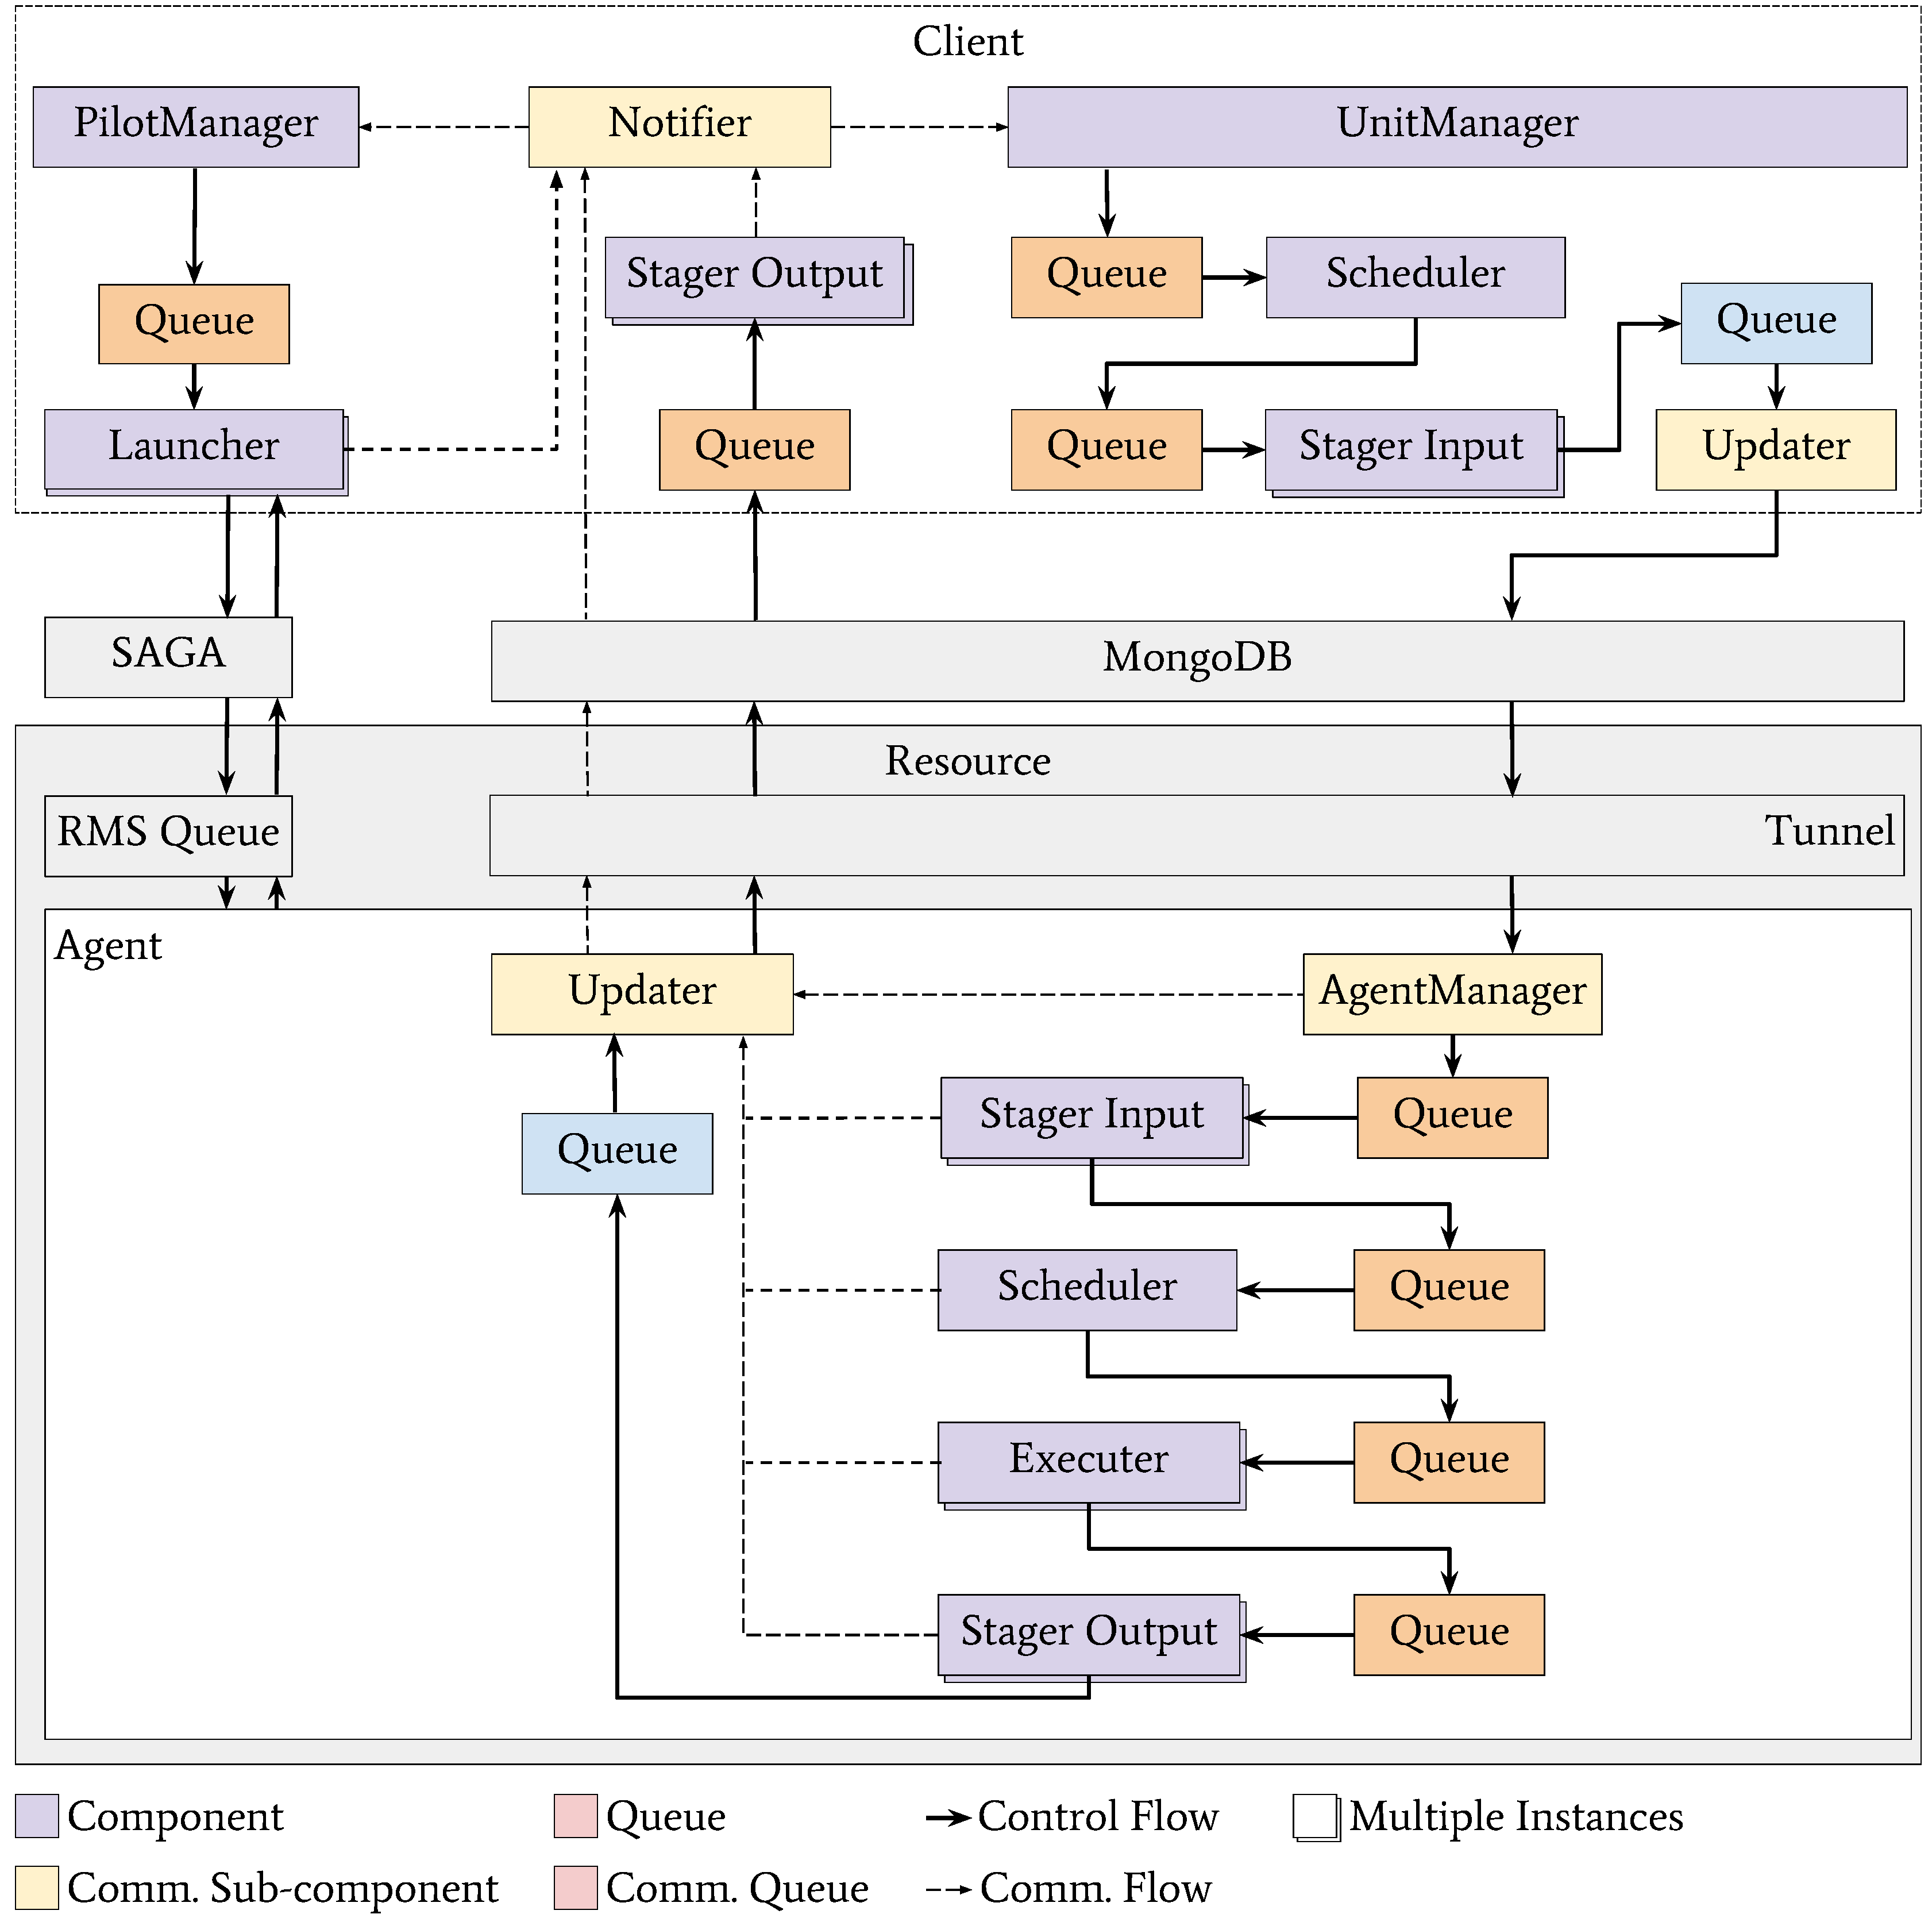
\includegraphics[width=0.58\textwidth]{figures/arch_rp.pdf} }}
    \qquad
    \subfloat[ ]{{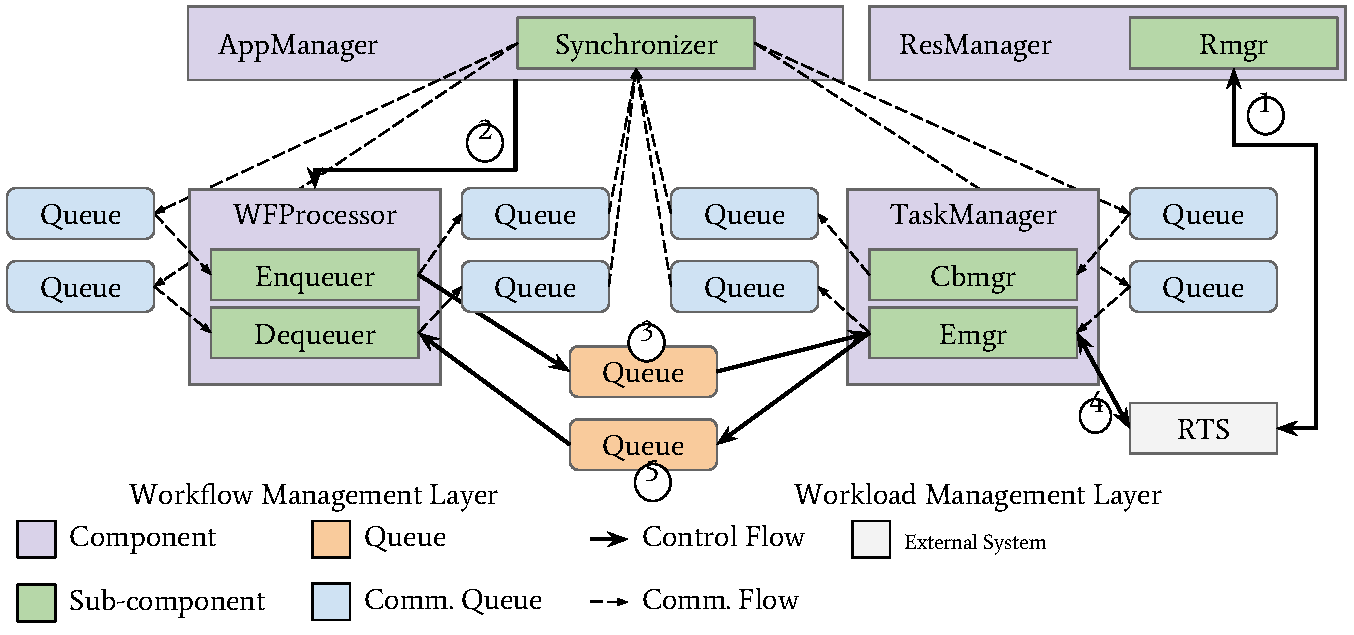
\includegraphics[width=0.32\textwidth]{figures/arch_entk.pdf} }}
    \caption{Caption. \mtnote{TODO\@: Fix EnTK AppManager}}\label{fig:archs}
\end{figure}

The first subsystem, called Client, has two main components designed to
manage either pilots or units: PilotManager and UnitManager. PilotManager has
a main component called `Launcher'. The Launcher uses resource configuration
files to define the number, placement, and properties of the Agent's
components of each Pilot. Currently, configuration files are made available
for all the HPC machines of the Extreme Science and Engineering Discovery
Environment (XSEDE), Blue Waters at the National Center For supercomputing
Applications (NCSA), Cheyenne at NCAR-Wyoming Supercomputing Center (NWSC),
and Rhea, Titan and Summit at the Oak Ridge National Laboratory (ORNL). Users
can provide new files or alter existing configuration parameters at runtime,
both for a single pilot or a whole RP session.

UnitManager has two main components: Scheduler and Stager Input. Scheduler
schedules compute units onto one or more pilots, available on one or more
resources. This enables late binding of units to resources, depending on
their availability: units are bound to resources that satisfy their execution
requirements only when these resources are actually available. The second
component of UnitManager is Stager Input. Units may need input files for
their execution, this module takes care to distribute these files to the
resources on which each unit has been scheduled.

The second subsystem of RP is called Agent and has four main components: one
Stager Input and Stager Output for staging input and output data of compute
units, Scheduler and Executer to schedule compute units on a pilot resources
and execute those units on them. Multiple instances of the Stager and
Executer components can coexist in a single Agent. Depending on the
architecture of the resource, the Agent's components can individually be
placed on cluster head nodes, MOM nodes, compute nodes, virtual machines, or
any combination thereof. ZeroMQ communication bridges connect the Agent
components, creating a network to support the transitions of the units
through components.

Data management \ldots\mtnote{Andre to write this paragraph about the
architectural specifics of data management in RP, mentioning Stager Output in
Client.}

Each component of each subsystem of RP has a dedicated queue. Orange queue in
Fig.~\ref{fig:archs}a are dedicated to pilots and unit entities while blue
queues to the messages exchanged by the components dedicated to
communication. Queuing entities enables managing them in bulk so to obtain
performance at scale in a distributed systems. Further, queuing entities
enables the use of concurrent components when using multiple physical
supports (e.g., work nodes) or when leveraging component concurrency for
performance optimization.

\mtnote{Introduce MongoDB and the role it plays for communication and
coordination.}

% ------------
\subsubsection{RADICAL Ensemble Toolkit}\label{sssec:arch_entk}

EnTK implements three main abstractions: task, stage and pipeline. Tasks
contain information regarding an executable, its software environment and its
data dependences. Stages are set of tasks where tasks have no mutual
dependences and can therefore execute concurrently, depending on resource
availability. Pipelines are lists of stages where a stage \(i\) can be
executed only after stage \(i-1\) has been executed.

The task abstraction identifies an executable as a program, not as an
instruction of a program. This is important: EnTK enables concurrent and
sequential execution at program-level, not at instruction level.
Instruction-level parallelism is still possible within each program run by an
EnTK task, enabling concurrent execution of multi-threaded, multi-process and
MPI programs. Note that. at the moment, EnTK requires a runtime system (RTS)
that support the same task abstraction.

Fig.~\ref{fig:archs}b shows the architecture of EnTK. The EnTK system (white)
has three components (purple), each with subcomponents dedicated to the
management of EnTK's entities (green) or coordination of the entities'
execution (yellow). The three components are AppManager, WFProcessor and
TaskManager that enable workflow specification, workflow execution
management, and workload management.

AppManager exposes an API for the development of ensemble-based applications
in terms of tasks, stages and pipelines, and for specifying resource
requirements for the application execution. AppManager initializes EnTK and
holds the global state of the application at runtime. AppManager is the sole
stateful component of EnTK, allowing to restart other components upon
failure, without interrupting the execution of the ensemble-based
application.

WFProcessor uses the Enqueue and Dequeue subcomponents to queue and dequeue
tasks pulled from AppManager. TaskManager uses ExecManager to schedule tasks
on the RTS and keep track of the state of each task during execution.
TaskManager users ResManageer as an interface to the chosen RTS. RTS have to
provide capabilities to acquire resources and schedule tasks on those
resources for execution. ResManager isolates RTS from EnTK, enabling
restarting of the RTS without loosing information about tasks that have been
already executed. Currently, EnTK support only RADICAL-Pilot as RTS but it is
designed to use other task-based RTS as, for example, Coasters or HTCondor.


% ---------------------------------------------------------------------------
\subsection{Software Functionalities}\label{ssec:functionalities}

{\em Present the major functionalities of the software.}

\begin{itemize}
  \item EnTK\@:
  \begin{itemize}
    \item Functionalities (VB)
  \end{itemize}
  \item RP\@: 
  \begin{itemize}
    \item Functionalities (AM)
  \end{itemize}
  \item RS\@:
  \begin{itemize}
    \item Functionalities (AM)
  \end{itemize}
  \item RA\@:)
  \begin{itemize}
    \item Functionalities (MT)
  \end{itemize}
\end{itemize}

% SAGA
Given the heterogeneity of distributed infrastructures, SAGA provides a much
needed interoperability layer that lowers the complexity and improves the
simplicity of using distributed infrastructure whilst enhancing the
sustainability of distributed applications, services and
tools.\mtnote{probably not to be included as SAGA has been already described
in a standalone SoftwareX publication.}

% RP
As a runtime system, RP offers an API to describe both pilots and CUs,
alongside classes and methods to manage acquisition of resources, scheduling
of CUs on those resources, and the staging of input and output files.
Reporting capabilities update the user about ongoing executions and profiling
capabilities enable detailed postmortem analysis of workload executions and
runtime behavior.

RP enables the execution of tasks with several dimensions of heterogeneity on
one or more pilots instantiated on one or more resources. The defining
capability of a pilot system is to decouple resource acquisition from task
execution. Infrastructures exposing resources via a batch system allow users
to submit their tasks as jobs. Jobs wait in the batch system's queue and when
the requested resources became available for the requested amount of time, a
job is scheduled for execution. Thus, each task of a multi-task application
has to wait in the batch system's queue to be executed, incurring in delays
that can become rapidly unfeasible.

Pilot systems allow for queuing a single job via the batch system and, once
this job becomes active, it executes a system application that enables the
direct scheduling of tasks on the acquired resources, without waiting in the
batch system's queue. In this way, pilot systems can enable high throughput
computing (HTC) on infrastructures designed to enable high performance
computing (HPC). Note that pilot systems do not game the HPC infrastructure:
pilot jobs are bound by the required resources and wait in the queue as every
other job, therefore abiding to the system usage policies.

RP offers four unique features when compared to other pilot systems or tools
that enable the execution of multi-task applications on HPC systems: (1)
concurrent execution of heterogeneous tasks on the same pilot; (2) support of
all the major HPC batch systems; (3) support of more than twelve methods to
launch tasks; and (4) a general purpose architecture. RP can execute single
or multi core tasks within a single compute node, or across multiple nodes,
isolating the execution of each tasks into a dedicated process and enabling
concurrent execution of heterogeneous tasks by design.

% EnTK
EnTK is a workflow engine specifically designed to execute ensemble-based
applications. These applications are composed by ensemble of tasks that may
have dependences both among tasks and ensembles. These dependences express a
relationship of priority at execution time. These dependences may be
determined by input/output data and control flow requirements: For example,
two tasks may have to be executed sequentially when the output of the first
task is the input of the second task; and two tasks (or ensembles) may have
to be executed sequentially when the output of the first tasks determines
whether executing the second task is of interest.

Consistently, EnTK provides adaptive capabilities and dedicated constructs to
pause, resume and stop pipelines at execution time. Adaptive applications
change the ensemble specifications at runtime, creating new pipelines, stages
and tasks, or changing the properties of those already described. Further,
pipelines and stages can be paused while waiting to perform \textit{ad hoc}
computations. This enable the implementation of high-level application
patterns as, for example, simulation-analysis, replica exchange and \ldots

% Execution Model

\mtnote{Describe BB and individual + aggregated execution models}


% ---------------------------------------------------------------------------
\subsection{Sample code snippets analysis (optional)}\label{ssec:code}

\begin{itemize}
  \item EnTK PST API
  \item RP pilot and unit API
\end{itemize}

% ---------------------------------------------------------------------------
% Section III
% ---------------------------------------------------------------------------
\section{Illustrative Examples}\label{sec:examples}

{\em Provide at least one illustrative example to demonstrate the major
functions.

Optional: you may include one explanatory video that will appear next to your
article, in the right hand side panel. (Please upload any video as a single
supplementary file with your article. Only one MP4 formatted, with 50MB
maximum size, video is possible per article. Recommended video dimensions are
640 x 480 at a maximum of 30 frames/second. Prior to submission please test
and validate your .mp4 file at $
http://elsevier-apps.sciverse.com/GadgetVideoPodcastPlayerWeb/verification$.
This tool will display your video exactly in the same way as it will appear
on ScienceDirect.).}

\begin{itemize}
  \item Simple EnTK application or one of the domain-specific workflows
  (HTBAC?) with RA analysis?
  \item Video of the execution because, why not?
\end{itemize}



% ---------------------------------------------------------------------------
% Section IV
% ---------------------------------------------------------------------------
\section{Impact}\label{sec:impact}

{\em \textbf{This is the main section of the article and the reviewers weight
the description here appropriately}

Guidelines for the authors:
\begin{enumerate}
  \item Indicate in what way new research questions can be pursued as a
        result of the software (if any).
  \item Indicate in what way, and to what extent, the pursuit of existing
        research questions is improved (if so).
  \item Indicate in what way the software has changed the daily practice of
        its users (if so).
  \item Indicate how widespread the use of the software is within and outside
        the intended user group.
  \item Indicate in what way the software is used in commercial settings
        and/or how it led to the creation of spin-off companies (if so).
\end{enumerate}}

% \begin{itemize}
%   \item Support of new research questions via RCT\@:
%   \begin{itemize}
%     \item General purpose pilot API, independent from domain, project,
%     infrastructure or middleware specific requirements.
%     \item General purpose task execution model: heterogeneous and.or
%     homogeneous set of tasks distributed across multiple
%     infrastructures/machines or distributed within a single machine. No
%     requirement for a specific distribution or communication pattern across
%     tasks.
%   \end{itemize}
%   \item Improved support of existing research question via RCT\@:
%   \begin{itemize}
%     \item Rapid codification of domain-specific applications due to
%     isolation of concerns between application logic and resource and
%     execution management.
%     \item Faster and simpler programmatic specification of tasks
%     dependences with the PST model.
%     \item User can control trade off between concurrency and duration of
%     the execution of multi-task applications (via pilots).
%     \item Strong and weak scaling on multiple HPC machines.
%   \end{itemize}
%   \item Impact on user practices:
%   \begin{itemize}
%     \item Writing domain-specific applications without having to
%     code/configure resource acquisition and execution management.
%     \item Rapid implementation of adaptive runtime strategies within
%     domain-specific applications.
%     \item Different modalities of deployment, including working for the
%     user workstation (or VM) without having to log into the computing
%     infrastructure.
%     \item Support of a large set of HPC machines via a unified and
%     consistent interface.
%   \end{itemize}
%   \item Adoption figures:
%   \begin{itemize}
%     \item Aggregated numbers for all RCT.
%     \item Break down figures?
%   \end{itemize}
% \end{itemize}

RCT have significant impact on several scientific projects, both as
individual and integrated systems. RCT are a testbed for engineering
research, mostly focused on foundational abstractions~\cite{}, architectural
paradigms~\cite{}, application patterns~\cite{}, and performance analysis of
distributed middleware on diverse computing infrastructures~\cite{}. RCT also
support several users worldwide, including individual researcher, research
laboratories and whole institutions. These users form a global community of
domain scientists and system engineers that actively contribute to the open
source development of RCT~\cite{}.

In the past five years, RCT has enabled the development of scientific
applications in multiple and diverse domains, including software engineering,
chemical physics, materials science, hearth science, climate science, drug
discovery and particle physics. RADICAL-SAGA and RADICAL-Pilot supports
several use cases, spanning functional and scientific domains. RADICAL-SAGA
is mostly integrated into end-to-end middleware solutions while RADICAL-Pilot
is used both as standalone system and integrated with other systems.

RADICAL-SAGA enables the Production ANd Distributed Analysis (PanDA) system
to submit batch jobs to Titan and Summit, the two leadership class machines
managed by the Oak Ridge Leadership Computing Facility (OLCF) at the Oak
Ridge National Laboratory (ORNL)~\cite{}. PanDA is the workload management
system used by the ATLAS project to execute hundred of millions of jobs a
year on both grid and High Performance Computing (HPC)
infrastructures~\cite{}. Only on ORNL, PanDA uses RADICAL-SAGA to analysis
more than eight million events a week.

RADICAL-SAGA was also used to develop Science Gateways as part of the
Distributed Application Runtime Environment (DARE) framework. These gateways
supported several projects, including DECIDE and neuGRID \mtnote{others?}, to
study the early diagnosis of Alzheimer and other neurodegenerative diseases.
In that capacity RADICAL-SAGA enabled submission of jobs to distributed
computing infrastructures managed by the European Grid Initiative (EGI),
interconnected via GEANT, the pan-European research and education network
that interconnects Europe’s National Research and Education Networks.

\mtnote{Other projects we should mention?}

As seen in Sec.~\ref{ssec:architecture}, RADICAL-PILOT uses RADICAL-SAGA to
submit pilots to a large array of resources, including HPC and grid systems
of the Extreme Science and Engineering Discovery Environment
(XSEDE)~\citep{towns2014xsede}, and the HPC machines Cheyenne at NCAR-Wyoming
Supercomputing Center (NWSC)~\citep{web-cheyenne}; Blue Waters at the
National Center For supercomputing Applications
(NCSA)~\citep{web-bluewaters}; Rhea, Titan and Summit at the Oak Ridge
National Laboratory (ORNL)~\citep{web-olcf-resources}; and SuperMUC at the
Leibniz Supercomputing Centre (LSC) of the Bavarian Academy of
Sciences~\citep{web-supermuc}.

Currently, RADICAL-Pilot (RP) supports fourteen projects across the USA and
Europe, for a total of \mtnote{insert number} collaborators. Since its first
release in \mtnote{add month and year}, RP has supported a total of
\mtnote{insert number} projects and \mtnote{insert number} collaborators. Of
these, \mtnote{insert number} projects used RP has a standalone system to
support the execution of multi-task applications on single and/or multiple
computing infrastructures. 

Among the most representative projects supported by RP as a standalone
system, the Abstractions and Integrated Middleware for Extreme-Scale Science
(AIMES) project enabled extreme-scale distributed computing via dynamic
federation of heterogeneous computing infrastructures. We used RP to execute
millions of tasks on both HPC and HTC resources, studying the federated
behavior of multiple infrastructures and progressing the foundational
understanding of the pilot abstraction and of the architectural pattern
underlying pilot systems.

\mtnote{Choose what other projects to add here for RP}

When EnTK, RP and RADICAL-SAGA are integrated into an end-to-end system, RCT
support the development of domain specific workflow (DSW) frameworks and
applications. DSW are \ldots

Currently, DSW frameworks like ICEBERG~\cite{}, HTBAC, RepEx, and EXTASY support the execution of workflows that share a specific coordination pattern. \ldots


% ---------------------------------------------------------------------------
% Section V
% ---------------------------------------------------------------------------
\section{Conclusions}\label{sec:conclusions}

{\em Set out the conclusion of this original software publication.}


% ---------------------------------------------------------------------------
% Acknowledgements
% ---------------------------------------------------------------------------
\section*{Acknowledgements}

{\em Optionally thank people and institutes you need to acknowledge. }

%% The Appendices part is started with the command \appendix;
%% appendix sections are then done as normal sections
%% \appendix

%% \section{}
%% \label{}


% ---------------------------------------------------------------------------
% References
% ---------------------------------------------------------------------------
\bibliographystyle{elsarticle-num} 
\bibliography{rct-softwarex}


% ---------------------------------------------------------------------------
% Appendix I
% ---------------------------------------------------------------------------
\section*{Required Metadata}\label{sec:metadata}


% ---------------------------------------------------------------------------
% Appendix II
% ---------------------------------------------------------------------------
\section*{Current code version}\label{sec:src_version}

{\em Ancillary data table required for subversion of the codebase. Kindly
replace examples in right column with the correct information about your
current code, and leave the left column as it is.

\begin{table}[!ht]
\begin{tabular}{|l|p{6.5cm}|p{6.5cm}|}
\hline
\textbf{Nr.}                                                     & 
\textbf{Code metadata description}                               & 
\textbf{Please fill in this column}                              \\
\hline
C1                                                               & 
Current code version                                             & 
For example v42                                                  \\
\hline
C2                                                               & 
Permanent link to code/repository used for this code version     & 
For example: $https://github.com/mozart/mozart2$                 \\
\hline
C3                                                               & 
Legal Code License                                               & 
List one of the approved licenses                                \\
\hline
C4                                                               & 
Code versioning system used                                      & 
For example svn, git, mercurial, etc. put none if none           \\
\hline
C5                                                               & 
Software code languages, tools, and services used                & 
For example C++, python, r, MPI, OpenCL, etc.                    \\
\hline
C6                                                               & 
Compilation requirements, operating environments \& dependencies & 
                                                                 \\
\hline
C7                                                               & 
If available Link to developer documentation/manual              & 
For example: $http://mozart.github.io/documentation/$            \\
\hline
C8                                                               & 
Support email for questions                                      & 
                                                                 \\
\hline
\end{tabular}
\caption{Code metadata (mandatory)}\label{tab:src_metadata} 
\end{table}}


% ---------------------------------------------------------------------------
% Appendix III
% ---------------------------------------------------------------------------
\section*{Current executable software version}\label{sec:bin_version}

{\em Ancillary data table required for sub version of the executable
software: (x.1, x.2 etc.) kindly replace examples in right column with the
correct information about your executables, and leave the left column as it
is.

\begin{table}[!ht]
\begin{tabular}{|l|p{6.5cm}|p{6.5cm}|}
\hline
\textbf{Nr.} & 
\textbf{(Executable) software metadata description} & 
\textbf{Please fill in this column} \\
\hline
S1 & 
Current software version & 
For example 1.1, 2.4 etc. \\
\hline
S2 & 
Permanent link to executables of this version  & 
For example: $https://github.com/combogenomics/$ $DuctApe/releases/tag/DuctApe-0.16.4$ 
\\
\hline
S3 & 
Legal Software License & 
List one of the approved licenses \\
\hline
S4 & 
Computing platforms/Operating Systems & 
For example Android, BSD, iOS, Linux, OS X, Microsoft Windows, Unix-like , IBM z/OS, distributed/web based etc. \\
\hline
S5 & 
Installation requirements \& dependencies & 
\\
\hline
S6 & 
If available, link to user manual - if formally published include a reference to the publication in the reference list & 
For example: $http://mozart.github.io/documentation/$ \\
\hline
S7 & 
Support email for questions & 
\\
\hline
\end{tabular}
\caption{Software metadata (optional)}
\label{tab:bin_metadata} 
\end{table}}

\end{document}
\endinput